\graphicspath{{content/chapters/literature_review/choosing_the_compositional_model/figures}}

\section{Choosing the Compositional Model}
\label{sec:choosing_the_compositional_model}

We will be exploring 3 compositional models which have been considered for this dissertation.
Each subsequent model builds upon the works of the former, adopting a more modular and understandable approach for solving \gls{vqa} tasks while also achieving better performance.

\subsection{Neural Module Network}
\label{subsec:neural_module_network}

The \gls{nmn} model\cite{andreas_deep_2016} is an attention-based compositional model which makes use of an array of \gls{nn} modules to solve \gls{vqa} tasks.
When given an image-question pair, it will predict an answer to the question using the following procedure:

\begin{itemize}\label{list:nmn_procedure}
    \item The image and question preprocessed, extracting their visual and textual features respectively.
    \item The image features, the question text, and the question features, are fed to the model as inputs.
    \item A new layout of \gls{nn} modules is created --- as seen in Figure~\ref{fig:nmn_overview} --- which is based upon the.
    \item The image features are inputted to each module, computing the output for each module.
    \item The text features are fed to an \acrshort{lstm}. Based on the input features, the outputs of only a specific set of the \gls{nn} modules will also be fed into the \acrshort{lstm}.
    \item The \gls{lstm} and layout outputs will averaged together to produce a final classification prediction as the answer to the input question.
\end{itemize}

\begin{figure}[htbp]
    \centering
    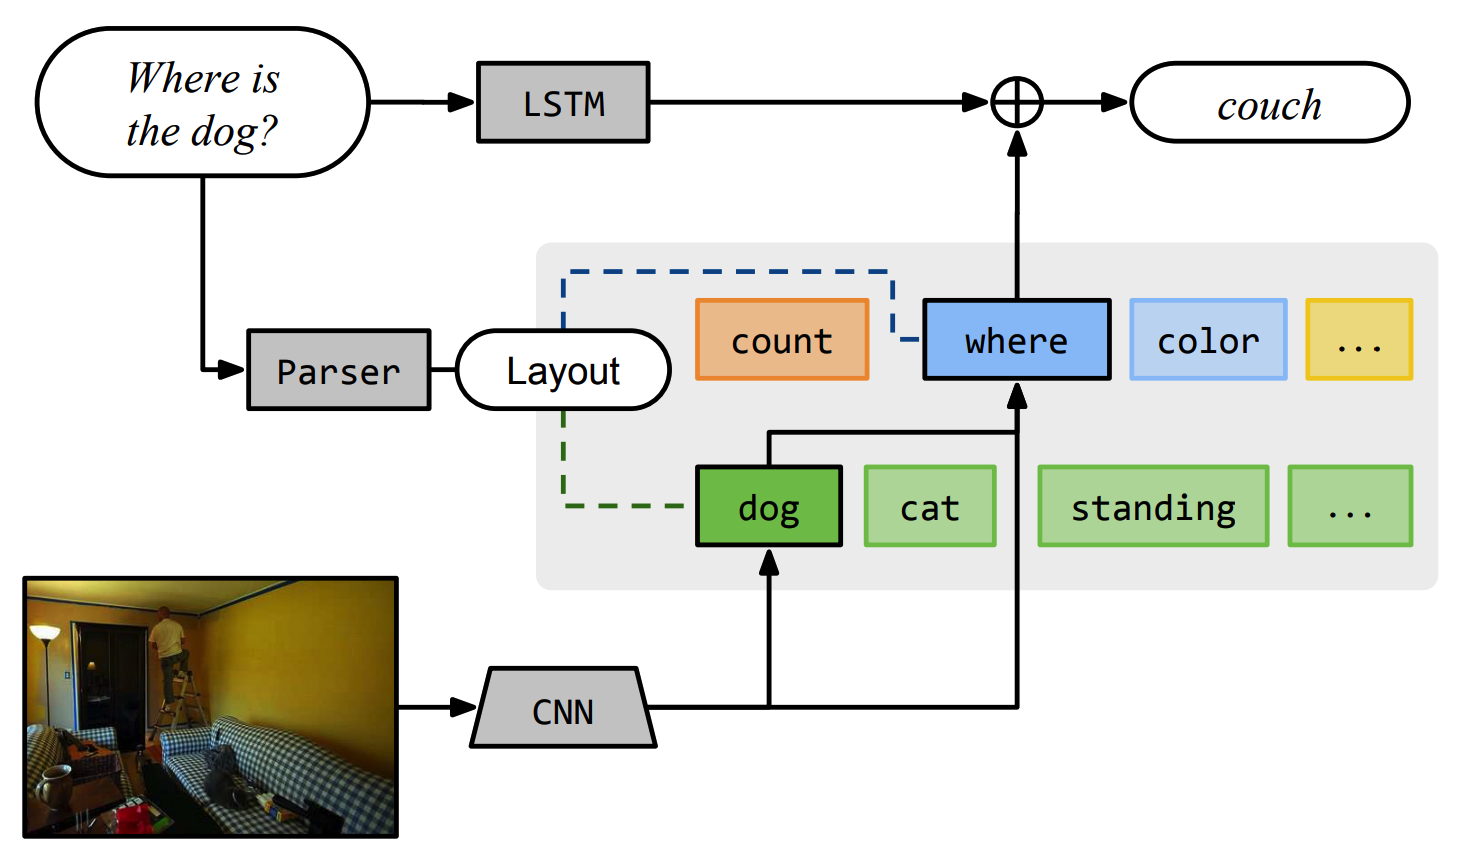
\includegraphics[width=.75\textwidth,keepaspectratio]{nmn_overview}
    \captionsource(\acrshort{nmn} Overview){How an \acrshort{nmn} predicts answers to a \acrshort{vqa} task. \label{fig:nmn_overview}}{\citeauthor{andreas_deep_2016}\cite{andreas_deep_2016}}
\end{figure}

Each module in the \gls{nmn} is described in the format \texttt{type[instance](arg1, ...)}, where \texttt{type} denotes the type of operation performed by the module (eg. \texttt{attend} will search for an object in the image) and \texttt{instance} identifies the module amongst other modules of the same type (eg. \texttt{attend[pillow]} identifies an \texttt{attend} module that looks for \texttt{pillow} objects in the image).
Arguments such as instance or type weights, or other argument types, are shared by the modules.
The paper introduced 5 module types for its \gls{nmn} model which can be found in Table~\ref{tab:nmn_module_list}.

\begin{table}
    \captionsource(\acrshort{nmn} module list){\acrshort{nmn} module types and example uses.\label{tab:nmn_module_list}}
    \centering
    \begin{tblr}{|c|c|c|c|}
        \hline
        \textbf{Module Name} & \textbf{Module label} & \textbf{Inputs \rightarrow Output} & \textbf{Example} \\
        \hline
        Attention       & \texttt{attend}       & Img \rightarrow Att       & \texttt{attend[ladder]}   \\
        Re-Attention    & \texttt{re-attend}    & Att \rightarrow Att       & \texttt{re-attend[right]}   \\
        Combination     & \texttt{combine}      & Att, Att \rightarrow Att  & \texttt{combine[include]} \\
        Classification  & \texttt{classify}     & Img, Att \rightarrow Lbl  & \texttt{classify[colour]}   \\
        Measurement     & \texttt{measure}      & Att \rightarrow Lbl       & \texttt{measure[count]}   \\
        \hline
    \end{tblr}
\end{table}

\begin{figure}[htbp]
    \centering
    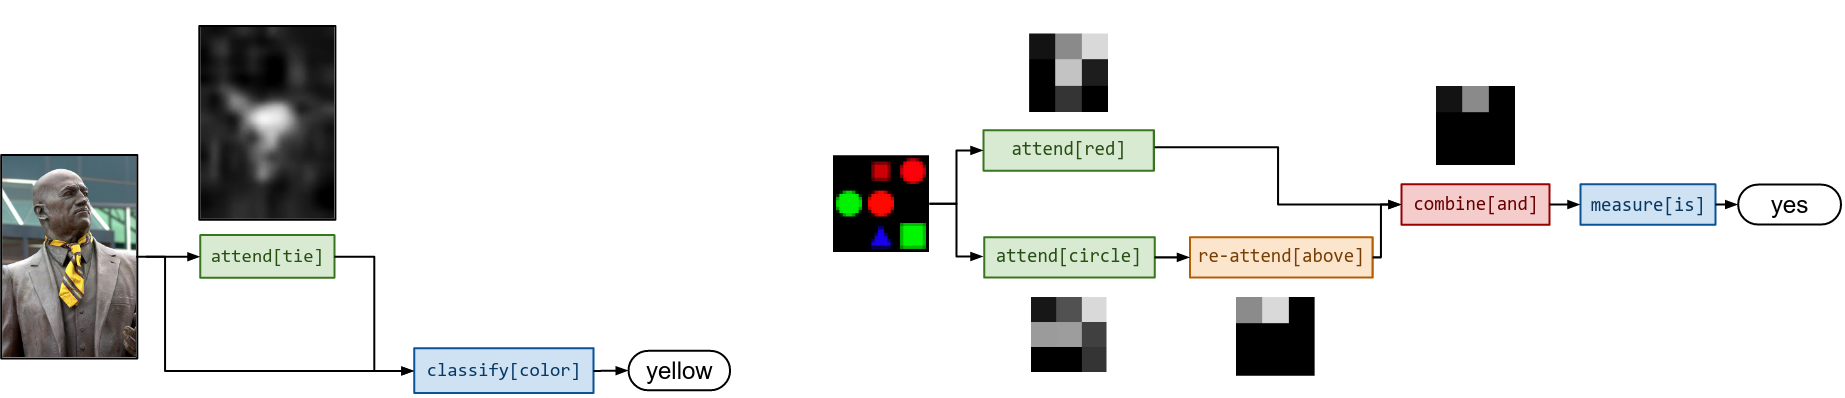
\includegraphics[width=\textwidth,keepaspectratio]{nmn_question_layout}
    \captionsource(\acrshort{nmn} layout construction){Example \acrshort{vqa} tasks being broken down by the \acrshort{nmn}. \textbf{Left:} Question: What colour is his tie? \textbf{Right:} Is there a red shape above a circle? \label{fig:nmn_question_layout}}{\citeauthor{andreas_deep_2016}\cite{andreas_deep_2016}}
\end{figure}

With the module instances prepared, the \gls{nmn} model now needs to know which module instances are required for each question.
To solve this, each question is converted into a layout, which identifies the modules required to answer the question.
To obtain these layouts, each question is first parsed using the Stanford Parser \cite{klein_accurate_2003}, a tool which uses a pre-trained language model to output standardised representations of the questions using the Universal Representations v1 format \cite{nivre_universal_2016}.
These representations are then simplified and converted into tokens which represent the module types and instances supported by the \gls{nmn} (for example: the question \texttt{"What is the colour of the cat left of the truck?"} could be converted into \texttt{"classify[colour](attend[cat](re-attend[left](attend(truck))))}").

While the above provides the model with a solid approach to predicting the answer, it will still be susceptible to errors due to overlooked grammatical cues in the question (such as \texttt{"What is swimming?"} versus \texttt{"What are swimming?"}; both questions denote the answer is something that's swimming, but the second question indicates a plural answer which cannot be represented or conveyed by the layouts protocol established above).
To solve this, the \gls{nmn} uses a \acrlong{lstm} question encoder to detect such cues, and combines its output with the output of the modules.
This effectively gives the final output of the model, the predicted answer to the image-question pair.

\begin{algorithm}
\captionsource(Pseudocode of \acrshort{nmn} solving \acrshort{vqa} task){A simplified pseudocode of how \acrshort{nmn} solves a \acrshort{vqa} task, from layout construction, to answer prediction.}{Original work written for this dissertation}\label{alg:nmn_solving_pseudocode}
\begin{algorithmic}[1]
    \State $img_o$ = raw image data \Comment{Original image}
    \State $q_o$ = "What colour is his tie?" \Comment{Original question}
    \State $img_f$ = GetImgFeatures($img_o$) \Comment{Convert to feature map}
    \State $q_{rep}$ = GetUDRepresentation($q_o$) \Comment{Get a Universal Dependency representation}
    \State $q_{func}$ = MapToFunctions($q_{rep}$) \Comment{"What colour is his tie" \rightarrow "colour(tie)"}
    \State $q_l$ = "" \Comment{Final network layout.}
    \ForAll{$w \in q_{func}$} \Comment{First "colour", then "tie"}
        \If{IsRoot($w$)}
            \State PushAnswerNode($q_l$, $w$) \Comment{Either 'measure' or 'classify' node}
        \ElsIf{IsLeaf($w$)}
            \State PushAttendNode($q_l$, $w$) \Comment{Always an 'Attend' node}
        \Else
            \State PushReAttentionNode($q_l$, $w$) \Comment{Either 'reattend' or 'combine' node}
        \EndIf
    \EndFor
    \State \Comment{$q_l$ is now "classify[colour](attend[tie])"}
    \State $a_{qe}$ = QEncoderPredictAnswer($q_o$) \Comment{Predict answer using \gls{lstm}}
    \State $a_l$ = LayoutPredictAnswer($q_l$) \Comment{Predict answer using layout and modules}
    \State \Comment{Get geometric mean of both predictions (layout-generated and \gls{lstm}-generated)}
    \State $a_{final}$ = $\sqrt[{2}]{a_{qe}a_{l}}$ \Comment{Final answer prediction.}
\end{algorithmic}
\end{algorithm}

\clearpage
\subsection{End-to-End Module Networks}
\label{subsec:n2nmn}

Building on the \acrshort{nmn} as an attention-compositional neural network, \citeauthor{hu_learning_2017} introduced \acrfull{n2nmn} as an \acrshort{nmn}-based model with an improved layout policy and network assembly \cite{hu_learning_2017} (See Figure~\ref{fig:n2nmn_overview}).

\begin{figure}[htbp]
    \centering
    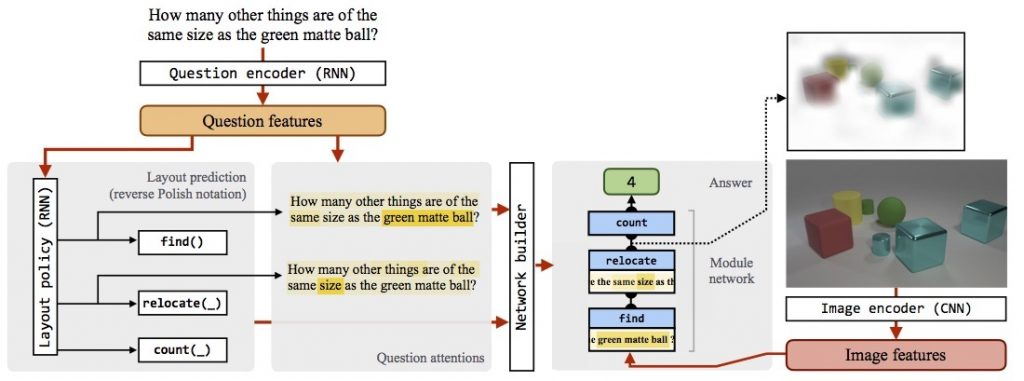
\includegraphics[width=\textwidth,keepaspectratio]{n2nmn_overview}
    \captionsource(\acrshort{n2nmn} model overview){The topology of the \acrshort{n2nmn} model, focusing on its approach to question representation and network layout assembly. \label{fig:n2nmn_overview}}{\url{https://ronghanghu.com/n2nmn/}}
\end{figure}

Similar to \acrshort{nmn}, \acrshort{n2nmn} uses neural modules which take one or two attention maps as input (depending on the module type) and outputs either another attention map or a probability distribution over the possible answers.
Aside from the given input maps, a module-specific textual vector --- obtained from the question being solved --- is also made available at runtime.
This textual vector is created by obtaining an attention map from word embeddings of each word in the question.
With this, a layout expression is created from which the \acrshort{n2nmn} is able to dynamically construct the modules needed using these textual vectors — as shown in Figure~\ref{fig:n2nmn_overview} — without relying on multiple separate, hard-coded module instances as is the case in the \acrshort{nmn} model.
An example breakdown of a question being answered --- with the modules used and their inputs/outputs shown --- can be seen in Figure~\ref{fig:n2nmn_layout_breakdown}.

\begin{figure}[htbp]
    \centering
    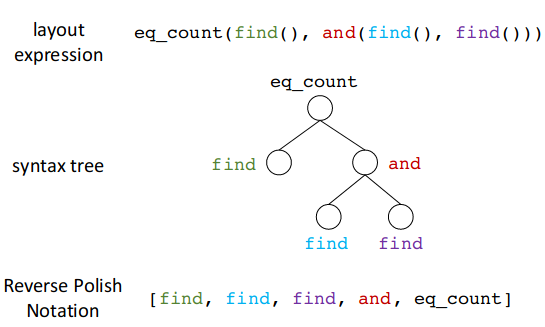
\includegraphics[width=.75\linewidth,keepaspectratio]{n2nmn_rpp}
    \captionsource(\acrshort{n2nmn} using \acrshort{rpp}){How \acrshort{n2nmn} constructs its layout policies using an \acrshort{rpp} sequence of module tokens. \label{fig:n2nmn_rpp}}{\citeauthor{hu_learning_2017}\cite{hu_learning_2017}}
\end{figure}

\begin{figure}[htbp]
    \centering
    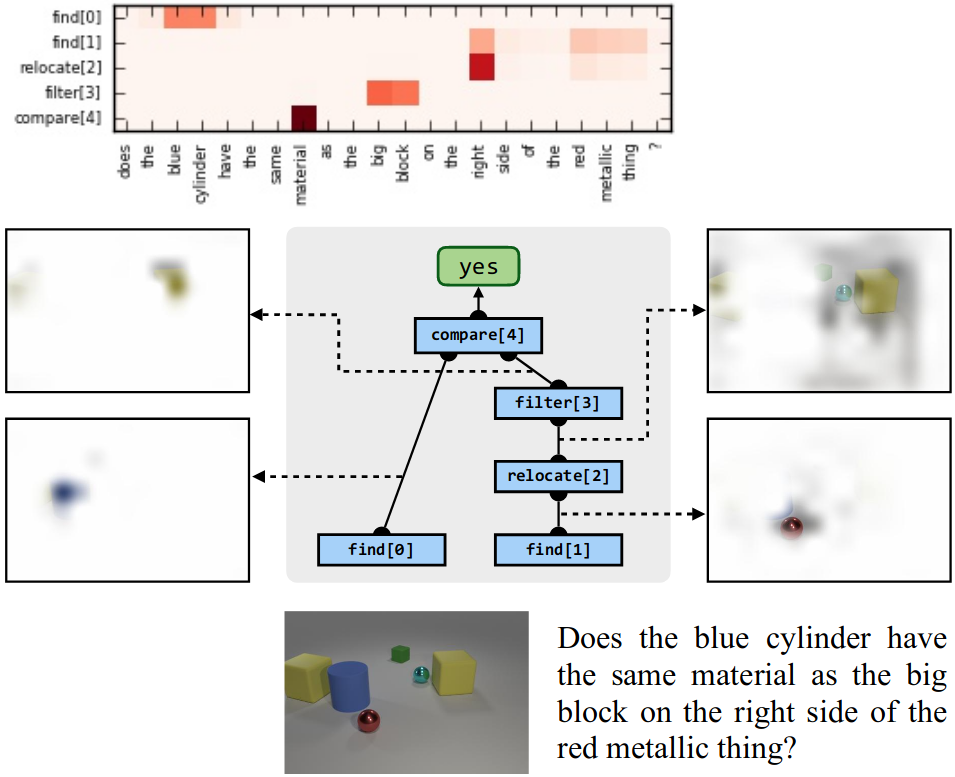
\includegraphics[width=.75\textwidth,keepaspectratio]{n2nmn_layout_breakdown}
    \captionsource(\acrshort{n2nmn} layout construction){A sample breakdown of a \acrshort{vqa} image-question pair, the textual attention for the question, the modules being called and their sequence, and the attentions being produced at each step.\label{fig:n2nmn_layout_breakdown}}{\citeauthor{hu_learning_2017}\cite{hu_learning_2017}}
\end{figure}

The layout expression is then converted into a sequence of module tokens using \acrlong{rpp} as shown in Figure~\ref{fig:n2nmn_rpp}. This has the benefit of representing the solution to predicting the answer as a series of smaller \acrshort{vqa} tasks.
The sequence is then parsed through an attentional \gls{rnn} \cite{bahdanau_neural_2016}. First, all words in the question are embedded into word vectors which are then fed into a multi-layer \gls{lstm}, outputting the encoded question as a vector of equal length.
An \acrshort{lstm} decoder then generates an attention map for the given encoder output and input words.
With this, a distribution of all possible layouts for the question can be predicted.
To narrow this down to the final layout, the model uses a beam search to select the best layout available from the distribution. From this, the final network is assembled.

During training, the layout policy and module parameters are jointly trained, using Adam for hyperparameter optimisation\cite{kingma_adam_2017}, and a loss function over the output answer scores to optimise these parameters.
Due to the layout policy being a discrete training problem, the loss function is not fully differentiable and does not allow for training with full back-propagation.
To circumvent this, those parts which are fully differentiable are trained with back-propagation, while those parts that aren't are trained using a policy gradient method optimised for reinforcement learning.

To optimise training of the layout policy, behavioural cloning is used to significantly reduce the starting loss of the model.
This is done by pre-training the layout policy against a previously-trained layout policy that gives viable performance (referred to as the expert policy).
Once trained, a suitable starting set of parameters are available to the sequence-to-sequence \gls{rnn} and the neural modules.
To avoid biasing of model performance on test sets, expert policies are only used when training on training sets.

\clearpage
\subsection{Stack Neural Module Network}
\label{subsec:stack_neural_module_network}

The \gls{n2nmn} model improved upon the original \gls{nmn}, but can still be improved further in ways that leverage its sequence-based architecture.
Succeeding the \gls{n2nmn} in performance and readability is the \gls{snmn} model, published by \citeauthor{hu_explainable_2019}\cite{hu_explainable_2019}.
The \gls{snmn} architecture is similar to that of \gls{n2nmn} with the exception of how its layouts are selected; whereas the \gls{n2nmn} layout policy selected a discrete set of modules in a layout, the \gls{snmn} layout controller uses a 'soft layout' where all modules are activated and their weighted outputs are averaged (See Figure~\ref{fig:snmn_overview}). The difference in layouts means the \gls{snmn} is fully-differentiable and trainable with back-propagation.

\begin{figure}[htbp]
    \centering
    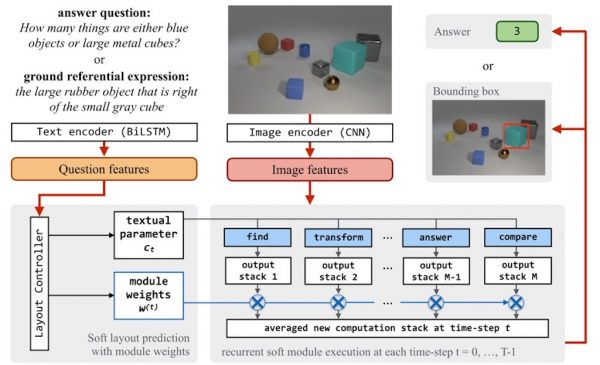
\includegraphics[width=.75\textwidth,keepaspectratio]{snmn_overview}
    \captionsource(\acrshort{snmn} model overview){The topology of the \acrshort{snmn} model and how it solves \acrshort{vqa} and \acrshort{ref} tasks. \label{fig:snmn_overview}}{\url{https://ronghanghu.com/snmn/}}
\end{figure}

The layout controller first encodes the input token sequence representing the question into a textual attention mask sequence representing the question by using a bi-directional \gls{lstm}.
The controller then uses an \acrshort{mlp} to predict a softmaxed attention vector containing a weight for each neural module in the model; this will be the soft layout.
In addition to the soft layout, a textual attention vector is then predicted for each token in the question sequence and used to predict the textual parameter which will be inputted to each module in the network.
The layout controller unrolls itself across all time-steps, repeating the above steps to produce a soft layout, textual parameter, and textual attention vector for each time-step.

\begin{table}
    \centering
    \begin{tblr}{|c|c|c|}
        \hline
        \textbf{Module Name} & \textbf{Inputs \rightarrow Output} & \textbf{Example} \\
        \hline
        \texttt{Find}       & (None) \rightarrow Att    & \texttt{Find['chair']()} \\
        \texttt{Transform}  & Att \rightarrow Att       & \texttt{Transform['left']()} \\
        \texttt{And}        & Att, Att \rightarrow Att  & Used internally \\
        \texttt{Or}         & Att, Att \rightarrow Att  & Used internally \\
        \texttt{Filter}     & Att \rightarrow Att       & \texttt{Filter['blue']()} \\
        \texttt{Scene}      & (None) \rightarrow Att    & Used internally \\
        \texttt{Answer}     & Att \rightarrow Ans       & \texttt{Answer['exist']()} \\
        \texttt{Compare}    & Att, Att \rightarrow Att  & \texttt{Compare['more']()} \\
        \texttt{NoOp}       & (None) \rightarrow (None) & Used internally \\
        \hline
    \end{tblr}
    \captionsource(\acrshort{snmn} module list){\acrshort{snmn} module types and example uses. Some modules are only used internally, or are used as part of the implementation of other modules.\label{tab:snmn_module_list}}{\citeauthor{hu_explainable_2019}\cite{hu_explainable_2019}}
\end{table}

Regarding modules, the \gls{snmn} uses the same module definitions as \gls{n2nmn} but simplified in implementation in some cases (See Table~\ref{tab:snmn_module_list} for a list of all implemented modules).
The main differences between the two implementations is that \gls{snmn} uses a single \texttt{Compare} module for comparison operations and an \texttt{Answer} module for tasks such as measuring or describing.
A \texttt{NoOp} module is also implemented which performs no computation or contribution to the predicted answer, but serves to pad out layouts should they finish before reaching the expected layout size.

Due to the input data requirements of some of the modules, the model needs to be able to provide data from one time-step to a module in a future time-step.
One example case being in \texttt{Compare(Find(), Transform(Find()))}, where the \texttt{Compare()} module needs to know the outputs of both the \texttt{Find()} module and \texttt{Transform()} module which were both executed in separate time-steps.
To address this, a memory stack is used to store outputs from intermediate neural modules where each module can then pop and push data onto the stack as needed.
The stack can store a pre-configured number of fixed-dimension vectors in its memory, while a one-hot vector - the same length as the stack - serves as the stack pointer.
The stack is designed to store image attention maps which are equal in size to the image feature maps.
Modules will then pop as many attention maps as needed and then push their output (if its an attention map) back onto the stack for other modules to use.
The model implements differentiable push and pop operations for manipulating the stack and its stack pointer.

When the model prepares to execute a layout, it begins by initialising the stack and setting the stack pointer to the 1st stack element.
From each time-step after initialisation, every module in the model is executed and popping any needed attention from the stack and pushing back onto the stack.
The result of each module is averaged together to produce a new stack representing the final state of that time-step, and the same averaging is performed on the stack pointer to indicate the top-most element at the end of the time-step.
The final output of the model is determined by averaging the weighted answer \glspl{logit} across all output modules (see Table~\ref{tab:snmn_module_list}) across all time-steps, and summing them to produce a final output \gls{logit}.

\subsection{Models comparison}
\label{subsec:models_comparison}

To discuss and compare the models discussed in \ref{sec:choosing_the_compositional_model}\nameref{sec:choosing_the_compositional_model} we will be focusing on their performance across all three datasets, discussing and elaborating on the performance metrics presented in Table~\ref{tab:model_performance_vqa}.
We will then follow up by highlighting the limitations of each model, and conclude by looking into how easy it is to understand the steps taken by each model to produce the results.

\begin{table}
    \centering
    \begin{tblr}{|l|c|c|c|c|}
        \hline
        \textbf{Model} & \textbf{SHAPES} & \textbf{CLEVR} & \textbf{VQAv1} & \textbf{VQAv2} \\
        \hline
        \gls{nmn}\cite{andreas_deep_2016} & 90.6 & 72.1\cite{hu_learning_2017} & 55.1 & - \\
        \gls{n2nmn}\cite{hu_learning_2017} & \textbf{100.0} & 83.7 & 64.9 (test-dev) & 63.3 \\
        \gls{snmn}\cite{hu_explainable_2019} & - & \textbf{96.5} & \textbf{66.0} & 64.0 \\
        \hline
    \end{tblr}
    \caption[{\acrshort{vqa} model performance across the \acrshort{vqa} datasets.}]{Comparison of models across the 3 \acrshort{vqa} datasets discussed. Results are measured in percentage accuracy (\%) and obtained from the highest-scoring run with all performance optimisations (such as expert layout) enabled. \label{tab:model_performance_vqa}}
\end{table}

Both \gls{nmn} and \gls{n2nmn} performed well on the SHAPES dataset, scoring 90.6\% and 100\% respectively.
While the images themselves are not complex at all - being only low-resolution images of 3-coloured 2d shapes - it served as a benchmark for testing the dynamics of a models layout-construction.
The questions are also yes/no questions meaning most of the performance may be carried by the models final stage which could be performing guesswork on the text of the question.
\gls{snmn} was not tested on this dataset so its performance isn't known, but could be assumed to be on-par with \gls{n2nmn} given the similarity in module implementation.

While the \gls{n2nmn} and \gls{snmn} both achieve scores of 83.7\% and 96.5\% on the CLEVR dataset respectively, the \gls{nmn} model was not tested on the dataset at the time of its publishing.
Despite this, it was modified to use the expert layout of the \gls{n2nmn} model so it would be able to train and test on the dataset, with which it was able to score 72.1\%\cite{hu_learning_2017}.
Since the dataset is arguably a more suitable dataset for testing layout-construction than SHAPES on account of it featuring the same complexity of questions, having more complex 3d scenes, it is assumed that \gls{nmn}

On the \gls{vqa}v1 dataset, \gls{nmn}, \gls{n2nmn}, and \gls{snmn} achieved test scores of 55.1\%, 64.9\%, and 66\%, respectively. Aside from those results, \gls{n2nmn} and \gls{snmn} were also tested on \gls{vqa}v2 and scored 63.3\% and 64.0\% respectively. Even when tested on natural images, the \gls{snmn} model remains effective, narrowly surpassing the \gls{n2nmn}.

Despite the performance of the \gls{nmn}, there are limitations concerning its ability to answer yes/no questions; as was suggested by \citeauthor{andreas_deep_2016}\cite{andreas_deep_2016}, the model seems to suffer from overfitting when training with yes/no questions.
Aside from this, the model uses hard-coded textual parameters which lead to measurably worse performance in the CLEVR dataset.
This problem does not occur in \gls{n2nmn} since the modules use soft-attention module parameters instead of hard-coded textual parameters.
Additionally, the \gls{n2nmn} seems to learn additional optimisations regarding how it attends to the image (such as in Figure~\ref{fig:n2nmn_layout_breakdown} where the second \texttt{find} module understands a subsequent re-attending of its output will look to the right of the image so the \texttt{find} attends to the left of the image).
The main drawback to the \gls{n2nmn} is its inability to use back propagation during training, instead relying on end-to-end training using reinforcement learning.
This limitation is addressed in the \gls{snmn} model, which is able to use back propagation during training thanks to its fully-differentiable layout controller and stack memory structure.
The \gls{snmn} model also seems to share the same optimisations seen in \gls{n2nmn} of composing a future time-step parameter into the current attention to optimise future time-steps.
Additionally, the \gls{snmn} model produces more human-interpretable results than the other models, and is supported by an experiment that was done comparing the \gls{snmn} model to a more closely-integrated model known as MAC\cite{hudson_compositional_2018} using human evaluators.
The model itself shared a very similar approach of using sequential time-steps with textual and visual parameters at each step, but does not use modular networks like the discussed models.
While the \gls{snmn} model was found to be more understandable and logically-predictable by human evaluators, its performance in the \gls{vqa} dataset was worse (by about 2\%) compared to the MAC model which was the state-of-the-art at the time\cite{hu_explainable_2019}.

When examining each of these models for ease of inclusion, all models are open-source, with their code-bases being released by the original authors.
The original \gls{nmn} model however, is discouraged for use by the original author who favours the newer \gls{n2nmn} model for being easier to set up and better performing\footnote{See \url{https://github.com/jacobandreas/nmn2/blob/master/README.md}}.
Building upon this, the \gls{n2nmn} and \gls{snmn} both share strong similarities in implementation, general architecture, and aims, with the main differences being that the \gls{snmn} uses a different memory structure and modified layout controller.
Aside from those, it also uses more recent versions of their dependencies which will help with development given the expected \acrshort{gpu} driver requirements for the specified dependency versions are no longer publicly available.
That said, the libraries used by the model are prior to a major version release, which may improve the performance of the model significantly but would necessitate a complete rewrite of the codebase.
Both these models use this legacy version so they ultimately would both require the same rewrite if done.
As a result of the reasons above, the benefits outlined in the discussion of results, 
and the ease of predictability of the model for human users who do not know the implementations of the model, the \gls{snmn} model will be chosen for this dissertation.

\clearpage
\subsection{Recognition to Cognition}
\label{subsec:recognition_to_cognition}

Having discussed and explored the above \gls{vqa} models, we will now explore a \gls{vcr} model to note the differences between the above \gls{vqa} models and this \gls{vcr} one.
The model chosen is the \gls{r2c} model\cite{zellers_recognition_2019}, introduced alongside the formal \gls{vcr} task declaration and the \gls{vcr} dataset\cite{zellers_recognition_2019}.
The model works differently to the compositional models seen above, using the following steps: \textbf{ground}, \textbf{contextualise}, then \textbf{reason}.

\begin{figure}[htbp]
    \centering
    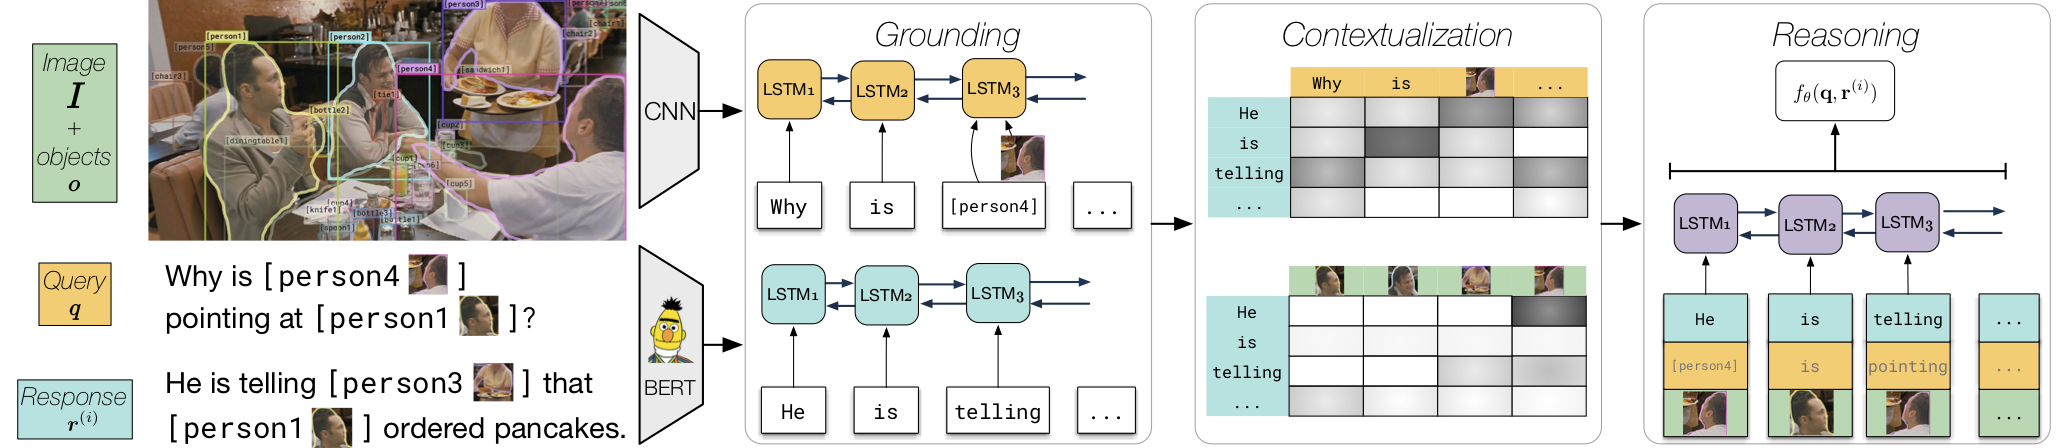
\includegraphics[width=\textwidth,keepaspectratio]{r2c_architecture_overview}
    \captionsource(\acrshort{r2c} model overview){Basic overview of the \acrshort{r2c} model and how it solves a \acrshort{vcr} task. \label{fig:r2c_architecture_overview}}{\url{https://github.com/rowanz/r2c/}}
\end{figure}

All image features are extracted using ResNet-50\cite{he_deep_2015} while language representations of the questions and responses are obtained using BERT\cite{devlin_bert_2019}.
The model is trained to reduce the multi-class cross entropy between the prediction of each response for the question, and the correct-most response.

When given a question-response pair, the model begins by \textbf{grounding} the question and response, by locating the objects in the image which are referenced.
By doing so, it derives the meaning of the question and the intention of each answer and rationale.
The grounding module begins by learning an image-language representation for the given tokens, which it shares for the question and responses (since they share the same vocabulary and tags).
Using this representation, the textual features of the question and responses are obtained.
Object features are then obtained by first using a \gls{cnn} over the image to obtain the initial object-level features and then combining with that object labels embedding in a shared hidden representation.
Both the object features and the textual features are fed into a bi-directional \gls{lstm} to produce the final outputs of the grounding module.

The outputs of the grounding module are then \textbf{contextualised} using the contextualiser module.
This performs a cross-multiplied softmax between the question, response, and object attentions to obtain the final contextualised representation of the question and the responses.

Finally, \textbf{reasoning} is performed by the model inside its reasoning module.
This is composed of a bidirectional \gls{lstm} which uses the contextualised representation of the question, object attentions, and responses, as input.
The output is then concatenated with the question and answer representations at each timestep for better gradient control by the loss function.
The final concatenated sequence is max-pooled, where an \gls{mlp} predicts a \gls{logit} representing confidence in the question-response pair.
